% Struttura concordata con il prof (mail del 29/10): introduzione (da scrivere per ultima),
% background, dataset, metodologia, esperimenti e risultati, conclusioni.
\documentclass[11pt,a4paper,twoside,openright]{book}
\usepackage[T1]{fontenc}
\usepackage[utf8]{inputenc}
\usepackage[italian,english]{babel}
\usepackage{csquotes}
\usepackage{lmodern}
\usepackage{amsmath,amssymb}
\usepackage{booktabs,array}
\usepackage{graphicx}
\usepackage{xcolor}
\usepackage[margin=2.8cm]{geometry}
\usepackage{caption}
\usepackage{enumitem}
\usepackage[style=numeric-comp,sorting=none,backend=biber,maxbibnames=8,giveninits=true,doi=false,isbn=false,url=true]{biblatex}
\usepackage[hidelinks]{hyperref}
\usepackage{bookmark}
\usepackage[capitalise,nameinlink]{cleveref}
\graphicspath{{figures/}}
% tikz/pgfplots per le figure: da aggiungere quando servono
\newcommand{\todo}[1]{\textcolor{red}{[TODO: #1]}}

% a tabular that is scaled down only when wider than the text width
\newsavebox{\fittablebox}
\newenvironment{fittable}{\begin{lrbox}{\fittablebox}}{\end{lrbox}%
  \ifdim\wd\fittablebox>\textwidth\resizebox{\textwidth}{!}{\usebox{\fittablebox}}\else\usebox{\fittablebox}\fi}

\addbibresource{bibliography.bib}
\begin{document}
\frontmatter
\begin{titlepage}
\centering

\includegraphics[width=3.4cm]{figures/cherubino}\par
\vspace{10pt}
{\LARGE\scshape Università di Pisa\par}
\vspace{6pt}
{\large Dipartimento di Ingegneria dell'Informazione\par}
\vspace{4pt}
{\large Master's Degree in Artificial Intelligence and Data Engineering\par}
\vfill
{\large\scshape Master's Thesis\par}
\vspace{18pt}
{\Large\bfseries Data Analysis and Data Mining\\on Decentralised Prediction Markets:\\[6pt]
the Price Process of Polymarket\\from One Minute to Twelve Hours\par}
\vfill
\begin{minipage}[t]{0.46\textwidth}
\raggedright
{\large\textbf{Supervisor}\\[6pt] Prof.\ Davide Bacciu\par}
\end{minipage}
\hfill
\begin{minipage}[t]{0.46\textwidth}
\raggedleft
{\large\textbf{Candidate}\\[6pt] Vito Pampinella\par}
\end{minipage}
\vfill
{\large Academic Year 2025/2026\par}
\end{titlepage}
\cleardoublepage

\chapter*{Abstract}
\addcontentsline{toc}{chapter}{Abstract}

This thesis studies Polymarket, a decentralised prediction market, as a data-analysis and
data-mining object: how twenty-one days of order-book, on-chain transaction and market
data were collected and prepared, what the price process and the transaction graph look
like, and which families of models can predict the direction of a market's price over
horizons from one minute to twelve hours.

\todo{rewrite at the end, together with the introduction}

\tableofcontents
% \listoffigures
% \listoftables
\mainmatter
\chapter{Introduction}
\label{ch:intro}

% da scrivere per ultima; la descrizione di Polymarket non va qui ma nel background
\todo{to be written last, once the other chapters are stable.  Only the outline for now.}

\section{Context}
\label{sec:intro:object}

Prediction markets as aggregators of dispersed information
\cite{wolfers2004prediction,arrow2008promise}; a decentralised one, Polymarket, exposes
the whole order book and every trade with the wallet behind it, at a resolution of about
two seconds, on tens of thousands of markets at once.  \todo{one page on why this is a
different object for a data scientist; the mechanics stay in \cref{ch:pm}}

\section{The problem}
\label{sec:intro:difficulty}

\todo{the task (direction of the mid price over one minute to twelve hours) and why it is
hard: a price consolidates information; it is bounded and discrete; it is mostly still;
much of what moves it is outside the data}

\section{Research questions}
\label{sec:intro:questions}

\begin{enumerate}[nosep,label=\textbf{Q\arabic*},ref=Q\arabic*]
  \item \label{q:process} What regularities does the price process of a prediction
  market have, and how is its trading organised?
  \item \label{q:information} Which publicly observable information predicts the
  direction of the mid price?
  \item \label{q:models} Which families of models can read that information, and what
  is a sequential state or a neighbourhood worth over a stateless learner on the same
  inputs?
  \item \label{q:horizon} How do the answers change with the horizon and with the kind
  of market?
\end{enumerate}

\section{Contributions}
\label{sec:intro:contributions}

\todo{list, once the results chapter is in place}

\section{Structure of the thesis}
\label{sec:intro:structure}

\todo{one paragraph per chapter}

\chapter{Background}
\label{ch:background}

% Polymarket: spostato dal vecchio capitolo e completato; i concetti di ML sono da scrivere
This chapter gives the background that the rest of the thesis assumes: what a prediction
market is and how Polymarket works (\cref{sec:pm:what,ch:pm}), and the notions of machine
learning that the methodology uses: time series and sequence models (\cref{sec:bg:ts}),
graphs and graph neural networks (\cref{sec:bg:graphs}), learners on tables of features
(\cref{sec:bg:tabular}) and evaluation under class imbalance (\cref{sec:bg:eval}).

\section{Prediction markets}
\label{sec:pm:what}

A prediction market trades contracts whose value is tied to the outcome of a future
event.  The simplest contract is the \emph{binary} one: it pays one unit if the event
happens and nothing otherwise.  If traders are risk-neutral and have no budget
constraints, the price of such a contract equals the market's aggregate probability of
the event; under weaker assumptions the price is still close to the mean belief of the
traders \cite{wolfers2004prediction,manski2006interpreting}.  Surveys of the empirical
literature find that market prices are well calibrated and competitive with polls and
expert forecasts, and that they react to news within minutes
\cite{wolfers2004prediction,snowberg2012prediction,arrow2008promise}.  Two
systematic deviations are documented: a favourite--longshot bias, where unlikely events
are over-priced and likely events under-priced, which grows with the time to expiration
\cite{page2013calibrated}; and, on Polymarket itself, the same bias
\cite{cardozo2026favorite} together with a concentration of trading profits in a very
small set of accounts \cite{akey2026whowins}.

\section{Polymarket}
\label{ch:pm}

\subsection{How Polymarket works}
\label{sec:pm:mechanics}

Polymarket is a decentralised prediction market built on the Polygon blockchain, with
the stablecoin USDC as collateral.  Every market is a question with two outcomes:
``Yes'' and ``No'' for a binary question, ``Up'' and ``Down'' for a price interval, the
two teams of a game, ``Over'' and ``Under'' for a total.  Each outcome is a conditional
token: one dollar of collateral can at any time be \emph{split} into one Yes token and
one No token, a pair can be \emph{merged} back into one dollar, and after resolution the
winning token is \emph{redeemed} for one dollar and the losing one for nothing.  The two
prices therefore sum to about one dollar, and a trader who wants to sell Yes at price $p$
is indistinguishable, for the matching engine, from one who wants to buy No at $1 - p$.

Trading takes place on a central limit order book that is \emph{hybrid}.  Orders are
signed messages that the trader submits to an off-chain operator, which keeps the book,
publishes every change to it and matches crossing orders; a match is then settled
on-chain by the exchange contract, which transfers tokens and collateral and emits a fill
event with the maker, the taker, the token, the side, the quantity, the price and the
fee.  The book is thus observable as a stream of price-level updates, and the trades as
on-chain records attributed to wallet addresses.  The two streams are not the same
thing: most book events are orders placed or cancelled away from the best quotes and never
trade; a fill is a book event that found a counterparty.

Multi-outcome events, the candidates of an election or the strikes of a ``Bitcoin above
$x$'' ladder, are sets of binary markets whose prices are linked by the payoff structure
(exactly one candidate wins), with a ``negative risk'' conversion that lets a trader hold
the No side of every candidate as one position.  The prices of such siblings must respect
bounds that the market does not always enforce \cite{gebele2026arbitrage}.

\subsection{Tokens, contracts and transactions: the blockchain layer}
\label{sec:pm:chain}

Polygon produces a block roughly every two seconds; every fill is a transaction in one
of its blocks and carries the block number, the transaction hash and the wallet
addresses of the maker and the taker.  Because settlement is on-chain, every trade is
attributed to a wallet that persists across markets and across time, which makes it
possible to build a bipartite graph between wallets and markets, and to ask whether the
history of a wallet (its activity, its past accuracy, the other markets it trades) is
informative about the price of the markets it trades now.  Works on Polymarket have used
wallet-level data to study who wins and who loses \cite{akey2026whowins}, insider trading
and informed flow \cite{bsic2026polymarket}, and arbitrage between related markets
\cite{saguillo2025unravelling}; none of them, to our knowledge, has used the wallet--market
graph as the input of a forecasting model, which is one of the questions of this thesis
(\cref{ch:graph}).  The block is also the natural time step of the on-chain stream, and it
is the time step of every stateful model in the thesis (\cref{sec:data:blocks}); the graph
itself is described in \cref{sec:expl:graph}.

\subsection{The limit order book}
\label{sec:pm:lob}

A limit order book \cite{gould2013limit} is, for one token, two sorted lists of resting
limit orders, bids and asks, each with the total size resting at that price.  The highest
bid and the lowest ask are the best quotes, their average is the \emph{mid price} and
their difference the \emph{spread}; the size at the first levels on each side is the
\emph{depth}.  Prices on Polymarket live in $[0, 1]$ with a tick of $0.001$ on most
markets, so a contract that is almost certain trades at $0.99$ or above and its price can
only move by a few ticks.  Because the Yes and No books mirror each other, the book of one
side describes the market, and this thesis reads the Yes side.  An \emph{order-book event}
is a change of the size resting at one price on one side; most events do not touch the
best quotes.  A \emph{snapshot} is the full state of the book at one moment.

Two consequences of this structure recur in every result of the thesis.  A mid price is a
bounded, discrete process observed through a thin book, so most of its changes are
one-tick oscillations produced by an order arriving at or leaving the best quote, which
are not information and which revert; and the dynamics depend on the price level, since a
market at $0.98$ has two ticks of room on one side and a hundred on the other.
\textcite{dubach2026anatomy} document the resulting microstructure on a 52-day sample:
depth depends on the market's duration, price level and volume and is spread over hundreds
of levels rather than concentrated at the top, and the trade direction inferred from the
public book matches the on-chain record only about 60\% of the time.  This is why the
thesis takes the direction of a trade from the on-chain fill and not from the book.

\subsection{The life of a market}
\label{sec:pm:life}

A market is created with its question, its resolution rules, its two outcomes and an end
date; its contract is deployed on-chain and it starts accepting orders at known times, both
recorded in the market's metadata and both known in advance.  It then trades until the
event is decided.  Some markets are born and die within minutes: the crypto interval
markets ask whether the price of Bitcoin, Ethereum or Solana will be above its starting
value at the end of a five- or fifteen-minute interval, and a new one opens as the previous
one closes; their prices follow an external reference, the spot price on a centralised
exchange, with a lag of a few hundred milliseconds \cite{young2026openmarket}.  Sports
markets trade before and during the game, with a recorded start time; political, economic
and cultural questions trade for weeks or months; daily temperature and weather questions
resolve every day.

Resolution is not decided by Polymarket.  When the event is over, a user proposes the
outcome to UMA's optimistic oracle and posts a bond in collateral; the proposal stands if
nobody disputes it within a two-hour challenge window, a wrong or premature proposal
forfeits the bond, and a disputed proposal goes through the oracle's dispute-resolution
process \cite{polymarket2026resolution}.  Resolution is therefore an event that happens
after the end date, sometimes well after it.  The thesis never uses the outcome or the
resolution time as an input: it predicts the price while the market is still open.
\todo{numbers on how many markets exist and how many are active per day, from
\cref{ch:data}}

\subsection{What is known about Polymarket}
\label{sec:pm:related}

Machine-learning work on Polymarket has so far concentrated on \emph{outcome}
forecasting with language models and news \cite{cheng2026polybench,barot2026polyswarm},
on dataset construction \cite{jia2026unlocking,young2026openmarket} and on the economics
of the platform \cite{reichenbach2025exploring,tsang2026anatomy}.
\textcite{young2026openmarket} is the closest in spirit: a logistic model on 43
order-flow features does not beat the Polymarket mid price itself as a predictor of the
outcome of the 15-minute Bitcoin markets.  The present thesis predicts the \emph{price},
not the outcome, over horizons at which the market is still open; the natural references
are therefore the limit-order-book forecasting literature (\cref{sec:bg:lob}) and the
literature on dynamic graphs (\cref{sec:bg:dyn}).  \todo{check whether anything else
came out on price (not outcome) forecasting}

\section{Time series, order books and sequence models}
\label{sec:bg:ts}

\subsection{Concepts}
\label{sec:bg:ts:concepts}

\todo{to write.  Outline:}
\begin{itemize}[nosep]
  \item time series; the order-book and transaction streams are sequences of timed
  \emph{events}, not series sampled on a regular grid;
  \item two ways of reading a stream: a fixed summary of the past handed to a learner
  without memory (\emph{stateless}), or a \emph{state} per market updated at every event
  (\emph{stateful}, recurrent); what each can see, how each is trained, how each handles
  irregular time;
  \item the task: the direction of the change over a horizon $H$, three classes
  (\textsc{down}, \textsc{const}, \textsc{up}); the random walk as the null model.
\end{itemize}

\subsection{Price predictability and limit order books}
\label{sec:bg:lob}

The efficient-market hypothesis in its weak form states that past prices carry no
information about future prices \cite{fama1970efficient}.  At short horizons this is only
approximately true: the stylised facts of high-frequency returns \cite{cont2001empirical}
include a negative autocorrelation at the shortest lags, produced by the bid--ask bounce
and by the discreteness of prices, and in a limit order book the next move of the mid is
related to the order-flow imbalance at the best quotes \cite{cont2014price}.
\todo{deep learning on limit order books, from DeepLOB \cite{zhang2019deeplob} on;
predictability depends on the microstructure more than on the architecture
\cite{briola2024deep}; one model pooled over many assets \cite{sirignano2019universal};
the warning about linear baselines \cite{zeng2023transformers}}

\subsection{Recurrent networks and multi-rate memories}
\label{sec:bg:rnn}

\todo{GRU \cite{cho2014gru} and truncated backpropagation through time; the clockwork RNN
\cite{koutnik2014clockwork} and GRU-D \cite{che2018grud} as the references of the
hierarchical memory and of the continuous-time decay}

\subsection{Time-series foundation models}
\label{sec:bg:tsfm}

\todo{Chronos and Chronos-2 \cite{ansari2024chronos,ansari2025chronos2}; the evidence in
finance, close to a random walk}

\section{Graphs and graph neural networks}
\label{sec:bg:graphs}

\subsection{Concepts}
\label{sec:bg:graphs:concepts}

\todo{to write.  Outline:}
\begin{itemize}[nosep]
  \item graphs; the bipartite graph between wallets and markets; degree, components,
  $k$-cores;
  \item dynamic graphs: a sequence of snapshots or a stream of timed events;
  \item message passing; on a bipartite dynamic graph, from wallets to the markets they
  trade and back.
\end{itemize}

\subsection{Graph neural networks}
\label{sec:bg:gnn}

\todo{message passing \cite{scarselli2009gnn,micheli2009nn4g,gilmer2017mpnn,bacciu2020gentle};
neighbourhood sampling and attention over the neighbours; a GRU as the node update
\cite{li2016ggnn}}

\subsection{Dynamic graphs}
\label{sec:bg:dyn}

\todo{continuous-time dynamic graphs \cite{kazemi2020survey,gravina2024dynamic}; the
memory-based models up to Temporal Graph Networks \cite{rossi2020tgn}; a model should
contain the strong heuristic as a special case \cite{feldman2026navis}}

\section{Gradient boosting and neural tabular learners}
\label{sec:bg:tabular}

\todo{LightGBM \cite{ke2017lightgbm} as the reference on tables of features; how a
neural tabular model has to be trained to compete
\cite{gorishniy2022embeddings,holzmuller2024betterbydefault}; TabM
\cite{gorishniy2025tabm}; logit adjustment under class imbalance
\cite{menon2021logitadjustment}}

\section{Evaluation under imbalance and dependence}
\label{sec:bg:eval}

\todo{balanced accuracy \cite{brodersen2010balanced}; dependent samples and the
hour-block bootstrap \cite{kunsch1989jackknife}; the focal loss \cite{lin2017focal}}

\chapter{The Dataset: Collection, Preparation and Exploration}
\label{ch:data}

% un unico capitolo: raccolta -> preprocessing -> dataset finale -> analisi esplorativa in chiusura
This chapter follows the data from their three sources to the objects the models read:
what was collected and from where (\cref{sec:data:sources,sec:data:collection}), how
large and how reliable it is (\cref{sec:data:scale,sec:data:quality}), how the raw
streams were preprocessed (\cref{ch:prep}) and how the final dataset was defined
(\cref{sec:data:final}).  It closes with an exploratory and statistical analysis of the
data (\cref{ch:exploration}).

\section{The four tables}
\label{sec:data:sources}

The dataset covers twenty-one consecutive days, from 6 to 26 March 2026, and consists of
four tables (\cref{tab:data:sources}).  The \emph{markets} table describes every market
that existed in the period: question text, tags, the two outcome tokens, creation and
end dates, and the final outcome.  The \emph{order book} table is the stream of
price-level updates of the ``Yes'' side of every market's book: each row carries the
best bid and ask, the changed price level, size and side, and the mid price.  The
\emph{snapshots} table holds full order-book states.  The \emph{transactions} table is
the on-chain record of every fill: block number, timestamp, transaction hash, wallet,
role (maker or taker), token, side, quantity, price and fee.

\begin{table}[t]
\centering
\caption{Data sources.  Row counts from the DuckDB database.}
\label{tab:data:sources}
\begin{tabular}{lrl}
\toprule
Table & Rows & Content \\
\midrule
markets      & 175{,}476            & one row per market: text, tags, tokens, dates, outcome \\
order book   & 5{,}555{,}777{,}555  & price-level updates of the Yes-side book \\
snapshots    & 51{,}674{,}425       & full order-book states (JSON) \\
transactions & 218{,}882{,}492      & on-chain fills with wallet, token, side, size, price \\
\bottomrule
\end{tabular}
\end{table}

\section{Collection}
\label{sec:data:collection}

\subsection{Market metadata: the Gamma API}

The \emph{markets} table was built from Polymarket's public metadata service (the Gamma
API): the markets closed in the window were paged through its keyset endpoint, and the
markets that appear in the transactions but not in that listing were completed one by
one through the markets-by-token endpoint.  The tags are the source of the eight
categories used throughout the thesis (crypto, sports, esports, politics, weather,
economy and tech, culture, other).

\subsection{The order-book archive}

The \emph{order book} and \emph{snapshots} tables come from a public archive of the
operator's websocket feed published on Kaggle \cite{gozo2026polymarket}: one file per
day, restricted to the Yes side of every book, with the creation time and the reception
time of every message.

\subsection{The on-chain transactions: a blockchain scraper}

The \emph{transactions} table was collected with a modified version of
\path{poly-trade-scan} \cite{martkir2026polytradescan}, an open-source client that reads
every Polygon block from a public node, filters the transactions addressed to
Polymarket's exchange contracts and decodes their \texttt{matchOrders} calls; the
modified version emits one row per wallet and per fill.  \todo{details of the decoding
(taker and maker legs, fees), the node, the retries; 219 million rows are fill legs}

\section{Scale, coverage and storage}
\label{sec:data:scale}

Daily activity is stable over the period: 9.2--11.8 million transaction rows,
122{,}000--161{,}000 distinct wallets and 15{,}000--21{,}000 active markets per day.
The data are stored as Parquet files and queried with DuckDB \cite{raasveldt2019duckdb}.
\todo{storage sizes; a figure of the daily volumes}

\section{Data quality}
\label{sec:data:quality}

\todo{the facts about the data that shape every later choice, with the numbers:}
\begin{itemize}[nosep]
  \item fabricated mid on one-sided books (the feature builder substitutes $0.49$ or
  $0.51$ for the missing side);
  \item token orientation: the book refers to token~1 in Yes/No markets and to token~2
  in all the others, while the raw trade direction refers to token~1 everywhere;
  \item about 40\% of the samples have a mid below $0.05$ or above $0.95$;
  \item one dip in the transaction stream, on 20 March.
\end{itemize}

\section{Preprocessing and audit of the pipeline}
\label{ch:prep}

\subsection{Time axis: blocks and the synchronisation of the two streams}
\label{sec:data:blocks}

Polygon produces a block roughly every two seconds, and every transaction carries its
block number.  The block is the time step of the models: a step is one block, the set
of transactions in it, and the order-book updates that arrived since the previous
block.  Because the two streams are collected by different clocks, a model that acts at
block $t$ sees every book update created strictly before $t$ and the fills of the block
itself.

\subsection{Derived tensors}
\label{sec:data:tensors}

\todo{to write:}
\begin{itemize}[nosep]
  \item a 52-dimensional feature vector per market and per order-book update (best
  quotes, five levels per side, spread, mid, imbalances, recent trade statistics),
  stored in hourly partitions;
  \item the market lifecycle table: deployment time (known in advance) and last trade
  (hindsight only, used to define the samples and never as an input);
  \item static market features: a sentence embedding of the question and a few
  numeric fields;
  \item dense indices for markets and wallets.
\end{itemize}

\subsection{Audit of the pipeline}
\label{sec:data:audit}

\todo{the three errors found by the audit and fixed before any result (wrong price
column; leaky momentum baseline; incomplete label lookup), and what was retrained}

\section{The final dataset: labels, samples, features and periods}
\label{sec:data:final}

\subsection{Labels}
\label{sec:data:labels}

The target of a market $m$ at block time $t$ and horizon $H$ is the sign of the change
of its mid price:
\begin{equation}
  y_{m,t} = \operatorname{sign}\bigl(\operatorname{mid}_m(t+H) - \operatorname{mid}_m(t)\bigr) \in \{\textsc{down}, \textsc{const}, \textsc{up}\},
  \label{eq:label}
\end{equation}
where $\operatorname{mid}_m(s)$ is the mid price of the last order-book update of $m$
strictly before $s$.  Three classes, because over one hour the mid of more than half of
the samples does not move at all; no dead zone, any move of at least one tick counts;
when $t + H$ is beyond the loaded data the label is missing.  \todo{samples: one per
(market, block) with an update; the deduplicated view, one sample per market per
fifteen minutes}

\subsection{Feature engineering}
\label{sec:prep:features}

\todo{to write.  The feature tables:}
\begin{itemize}[nosep]
  \item the sixty-one hand-made causal features, in five groups: price history, book
  shape, activity and clock, on-chain trades, static fields of the market (the full
  list in \cref{app:features});
  \item sibling features: the contracts of the same event;
  \item news features: GDELT counts and tone for the entities named in the question;
  \item wallet features on the transaction edges;
  \item forecast features: the quantiles of a zero-shot Chronos-2 forecast.
\end{itemize}

\subsection{Training, validation and test periods}
\label{sec:data:splits}

The twenty-one days are split by date: models are trained on 6--12 March and every
design choice is taken on the validation day, 13 March; the period 24--26 March is a
locked test set, never evaluated and never inspected, reserved for the final numbers.

\section{Exploratory and statistical analysis}
\label{ch:exploration}

\todo{in closing, as agreed: what the data say before any model is trained, in three
parts.  Numbers on the training and validation days only.}

\subsection{The price process}
\label{sec:expl:price}

\todo{outline: the event stream and how uneven it is; how often a price moves at each
horizon (\cref{tab:expl:classes}); the price level; the activity clock; the direction
of a move; the kind of contract; the contracts of the same event; the wallets}

\begin{table}[t]
\centering
\caption{Share of the three classes among the labelled validation samples, by horizon.}
\label{tab:expl:classes}
\begin{tabular}{lccc}
\toprule
Horizon & \textsc{down} & \textsc{const} & \textsc{up} \\
\midrule
1 min  & 0.057 & 0.891 & 0.052 \\
15 min & 0.164 & 0.690 & 0.146 \\
1 h    & 0.236 & 0.549 & 0.215 \\
6 h    & 0.335 & 0.354 & 0.312 \\
12 h   & 0.377 & 0.275 & 0.348 \\
\bottomrule
\end{tabular}
\end{table}

\subsection{The transactions as a graph}
\label{sec:expl:graph}

\todo{size, density and degree distributions; components and $k$-cores; the graph in
time; a map of the graph (\cref{fig:graph:map:cat}); synchronous publics; what it says
for the models}

\begin{figure}[p]
\centering
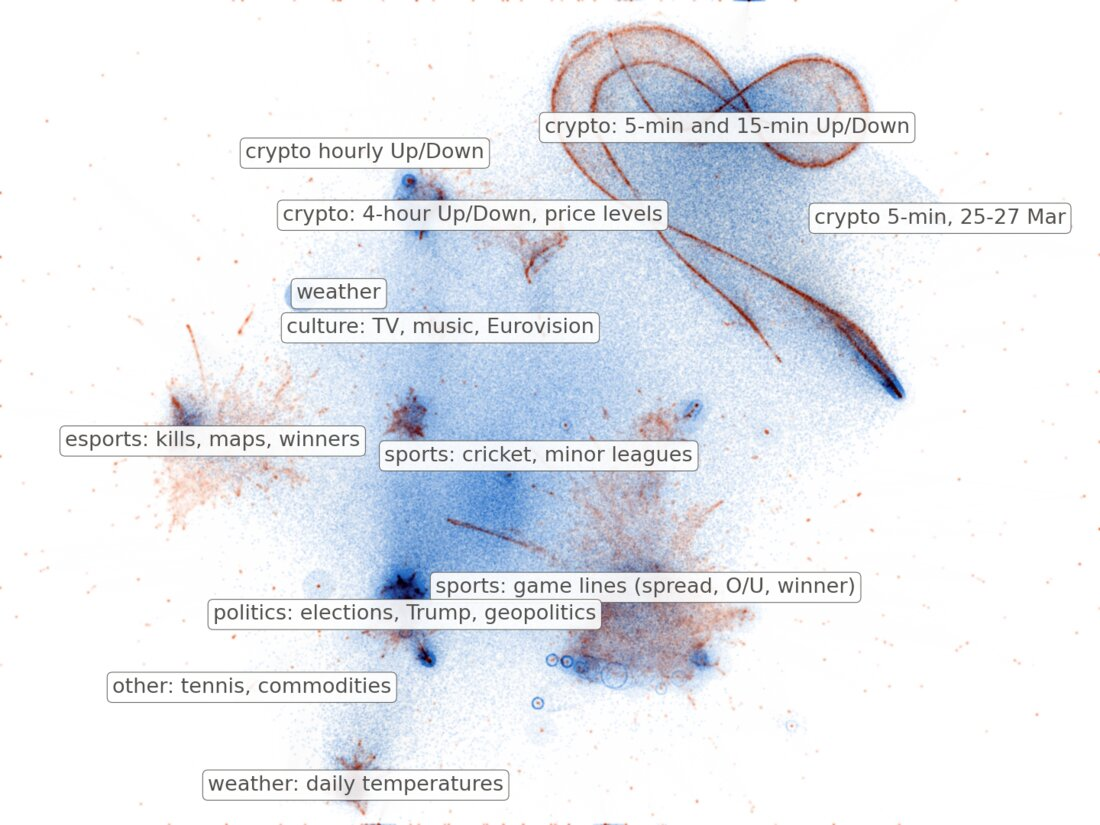
\includegraphics[width=\textwidth]{figures/graph/graph_map_category.jpg}
\caption{Three weeks of transactions as a graph: wallets (blue) and markets (orange),
joined by the trading relations between them, 6--26 March 2026.  \todo{caption}}
\label{fig:graph:map:cat}
\end{figure}

\subsection{The structure of the feature space}
\label{ch:structure}

\todo{data-mining study of the hand-made features: how many quantities they contain
(PCA, correlation blocks); maps of the samples (UMAP, t-SNE); linear, local and
threshold separability; families of markets; across the horizons}

\subsection{What the data say before a model is trained}
\label{sec:expl:agenda}

\todo{summary that sets the agenda of the methodology}

\chapter{Methodology}
\label{ch:models}

% razionale (obiettivo, criteri, regole di inclusione) + famiglie di approcci con pro e contro
This chapter sets out the rationale of the study (\cref{sec:meth:rationale}) and the
approaches that were compared, in five families: causal rules on the price, stateless
learners on hand-made features, sequence models of the order-book stream, graph models,
and sources of information outside the book.  \todo{each family closes with its
advantages and limits a priori; a summary table at the end}

\section{Objective, criteria and rules of inclusion}
\label{sec:meth:rationale}

\subsection{Objective}
\label{sec:meth:objective}

The object of the study is the direction of the mid price of a Polymarket market over a
horizon $H$, read as the three-class label of \cref{sec:data:labels}, at every block in
which the market updated its book, for five horizons from one minute to twelve hours.
The task is the prediction of the price while the market is open, not of the outcome of
the event; the measure is balanced accuracy, because the three classes are of very
unequal size and change size with the horizon; and the unit of every comparison is the
paired difference between two models on the same samples, with an interval.

\subsection{Criteria of success}
\label{sec:meth:criteria}

A model is said to read information that another does not when its balanced accuracy
on the validation day exceeds the other's on the same samples, after the same post-hoc
calibration, by a margin whose 95\% hour-block bootstrap interval excludes zero.  The
reference competitor is first the best causal rule found on the data and then, once it
exists, the best stateless learner on hand-made features.  \todo{ties; the two views of
the samples (full stream and deduplicated); the locked test period}

\subsection{Rules of inclusion and exclusion}
\label{sec:meth:rules}

\todo{to expand, one paragraph each:}
\begin{enumerate}[nosep]
  \item \textbf{Causal inputs only.}  Everything an approach reads at time $t$ is
  computed from data strictly before $t$, and every label from data after it.
  \item \textbf{Public information that the dataset contains}, plus two public external
  sources that could be aligned to it (the news flow, a pretrained forecaster); no
  external reference prices.
  \item \textbf{One model for all markets}, never one model per market.
  \item \textbf{Every approach is measured against the best simpler one on the same
  inputs}, and where possible contains it as a special case.
  \item \textbf{Families that span the questions}: each research question has a paired
  comparison.  Out of scope: outcome forecasting with language models, trading
  strategies, per-market models.
  \item \textbf{A fixed compute budget}: one run per GPU, hours per run; short tests to
  screen the variants, full-length runs behind every claim.
\end{enumerate}

\section{Baselines: causal rules on the price}
\label{sec:models:baselines}

All baselines are causal rules on the mid price of the market itself.  With
$\Delta^{-}_{L} = \operatorname{mid}(t) - \operatorname{mid}(t-L)$ the change over the
past lookback $L$:
\begin{itemize}[nosep]
  \item \textbf{Constant}: always \textsc{const}; balanced accuracy $1/3$ by construction.
  \item \textbf{Momentum-$L$}: predict $\operatorname{sign}(\Delta^{-}_{L})$.
  \item \textbf{Mean Reversion-$L$}: predict $-\operatorname{sign}(\Delta^{-}_{L})$, and
  \textsc{const} if the price did not move.
\end{itemize}

\paragraph{Advantages and limits.}  \todo{to write}

\section{Stateless learners on hand-made features}
\label{sec:models:stateless}

A LightGBM classifier \cite{ke2017lightgbm} on the sixty-one features of
\cref{sec:prep:features}, trained with class-balanced weights on 7--11 March and
early-stopped on 12 March, adding one group of features at a time.  On the same table,
an MLP and a TabM ensemble, trained as tabular models should be (\cref{sec:bg:tabular}),
to tell whether a difference between the trees and a deep model is the learner or the
training regime.  \todo{hyper-parameters}

\paragraph{Advantages and limits.}  \todo{to write}

\section{Sequence models of the order-book stream}
\label{sec:models:sequence}

\subsection{The continuous-time stateful model}
\label{sec:models:ctdgnn}

The model (CT-DGNN in the code) processes the stream block by block.  At block time $t$
it receives the markets that updated their book since the previous block, with a window
of their last $K$ book states, and the transactions of the block as edges between
wallets and markets; it keeps a state vector for every market and every wallet.
\todo{one step of the model, with the architecture figure from the old chapter:}
\begin{itemize}[nosep]
  \item states and initialisation; continuous-time decay of the states;
  \item order-book update: the window encoders (space first, or time first);
  \item hierarchical memory at three rates; global state;
  \item long-lookback price features and the direct path, which contains the
  mean-reversion rule as a special case;
  \item predictor, loss and training (truncated BPTT, one pass through the stream).
\end{itemize}

\subsection{The stateful model as the residual of the trees}
\label{sec:models:residual}

\todo{cross-fitted tree log-probabilities added to the output logits; at initialisation
the model is the tree model, and the number that measures the state is the gain over it}

\subsection{A pretrained forecaster used zero-shot}
\label{sec:models:zeroshot}

\todo{Chronos-2 on the last 512 mids of the market; three decision rules; the same
quantiles as features of the stateful model}

\paragraph{Advantages and limits.}  \todo{to write}

\section{Graph models}
\label{sec:models:graph}

\subsection{Message passing on transactions}
\label{sec:models:mp}

\todo{edges $(w, m)$ with a 7-dimensional feature; attention over the incident edges
and a GRU update; the token-orientation feature; the enrichments (wallet skill, placebo
skill, past behaviour); the ablation without edges}

\subsection{The two graphs}
\label{sec:models:twographs}

\todo{the wallet--market graph, read by message passing, and the market--market graph
between the contracts of the same event, measured first through the sibling features}

\paragraph{Advantages and limits.}  \todo{to write}

\section{Information outside the book}
\label{sec:models:external}

\todo{the foundation-model forecasts, the news flow, the text of the market; each
measured first in the stateless learner}

\paragraph{Advantages and limits.}  \todo{to write}

\section{The families at a glance}
\label{sec:models:summary}

\todo{table: family, members, what it reads, where its state lives, reference}

\chapter{Experiments and Results}
\label{ch:experiments}

% da riorganizzare per famiglia nell'ordine del cap. 4; finora spostati setup e regole causali
\todo{the results of the old chapters, reorganised by family in the order of
\cref{ch:models}; only the setup and the causal rules moved so far}

\section{Experimental setup}
\label{sec:data:protocol}

Models are trained on 6--12 March and validated on 13 March, with 24--26 March locked
for the final numbers.  All numbers are balanced accuracies on the validation day,
reported on all samples and on three subsets: the \emph{deduplicated} samples (at most
one per market per fifteen minutes), the \emph{extreme} ones (mid outside
$[0.05, 0.95]$) and the \emph{central} ones.  Differences between models are computed on
exactly the same samples and carry a 95\% hour-block bootstrap interval.  \todo{the
three rules that make the comparisons fair: the same samples; the same post-hoc
calibration (two logit offsets, cross-fitted on the validation hours); full-length runs
behind every claim.  Compute: one run per GPU, hours per run.}

\section{Rules and stateless learners}
\label{ch:stateless}

\subsection{Causal rules}
\label{sec:stateless:rules}

\begin{table}[t]
\centering
\caption{Causal rules on the validation day, balanced accuracy, all samples and
deduplicated samples.  Momentum-$H$ and Mean Reversion-$H$ use the change over the past
$H$; Momentum last-tick uses the sign of the last mid change.}
\label{tab:exp:baselines}
\small
\begin{fittable}\begin{tabular}{lcccccccccc}
\toprule
& \multicolumn{2}{c}{1 min} & \multicolumn{2}{c}{15 min} & \multicolumn{2}{c}{1 h} & \multicolumn{2}{c}{6 h} & \multicolumn{2}{c}{12 h} \\
\cmidrule(lr){2-3}\cmidrule(lr){4-5}\cmidrule(lr){6-7}\cmidrule(lr){8-9}\cmidrule(lr){10-11}
Rule & all & dedup & all & dedup & all & dedup & all & dedup & all & dedup \\
\midrule
Constant                  & 0.333 & 0.333 & 0.333 & 0.333 & 0.333 & 0.333 & 0.333 & 0.333 & 0.333 & 0.333 \\
Momentum last-tick        & --- & --- & --- & --- & 0.375 & 0.387 & 0.365 & 0.374 & 0.362 & 0.370 \\
Momentum-$H$              & --- & --- & --- & --- & 0.472 & 0.445 & 0.436 & 0.422 & 0.424 & 0.420 \\
Mean Reversion-$H$        & \textbf{0.536} & \textbf{0.501} & \textbf{0.537} & \textbf{0.525} & \textbf{0.527} & \textbf{0.506} & \textbf{0.501} & \textbf{0.488} & \textbf{0.507} & \textbf{0.500} \\
\bottomrule
\end{tabular}\end{fittable}
\end{table}

Mean Reversion-$H$ is above $0.5$ at every horizon and it is the rule to beat
(\cref{tab:exp:baselines}); Momentum is far below it.  \todo{why mean reversion is
strong: a bounded, discrete price whose moves are mostly one-tick oscillations that
revert}

\subsection{Trees on hand-made features: the no-state control}
\label{sec:stateless:control}

\todo{the table by feature group at one hour; the other horizons; where the information
is}

\subsection{Neural tabular learners: trees against networks}
\label{sec:stateless:tabular}

\todo{MLP and TabM against LightGBM, three seeds}

\section{Stateful models}
\label{ch:stateful}

\todo{from the first models to the last: the retraining on the correct target; loss and
imbalance variants; memory, direct path and lookbacks; the window encoders; the state
given the control's inputs; the cost of the online regime; the residual of the trees;
what the state is worth}

\section{Graph models}
\label{ch:graph}

\todo{the wallet--market graph at every stage of the design; smart money; the sibling
contracts; why the graph does not help}

\section{Information outside the book}
\label{ch:external}

\todo{foundation models zero-shot and as features; news volume; the text of the market}

\section{Across horizons, kinds of market and seeds}
\label{ch:horizons}

\todo{one and fifteen minutes; one hour; six and twelve hours; the synthesis table; by
kind of market; robustness (seeds, calibration, short tests against full runs)}

\section{Test set}
\label{sec:horizons:test}

\todo{final numbers on 24--26 March, produced once at the end}

\section{Discussion}
\label{sec:horizons:questions}

\todo{the results against the four questions of \cref{sec:intro:questions}}

\chapter{Conclusions}
\label{ch:conclusions}

\todo{after the results chapter}

\section{What the thesis found}
\label{sec:concl:summary}

\todo{question by question}

\section{Limitations}
\label{sec:concl:limits}

\todo{to write}

\section{Future work}
\label{sec:concl:future}

\todo{to write}

\appendix
\chapter{The hand-made features}
\label{app:features}

\todo{table of the sixty-one features, one line each, with the definition and the group (price history, book shape, activity and clock, trades, static)}

\backmatter
\printbibliography[heading=bibintoc]
\end{document}
